\section{S2 -- HTML DOM i XHTML -- cel i charakterystyka}

\subsection{HTML (HyperTextMarkup Language)}

\textbf{Cel:}
\begin{itemize}
\item Zapewnienie uniwersalnego, przenaszalnego, niezależnego od platformy sprzętowej i systemu operacyjnego standardu opisującego struktury strony internetowej;
\item Nadanie elementom strony odpowiedniego znaczenia semantycznego strony w zależności od ich zawartości np. tag \texttt{<em>};
\item Umożliwienie pozycjonowania strony w wyszukiwarkach internetowych w zależności od zawartości strony np. tag \texttt{<article>}
\end{itemize}

\textbf{Charakterystyka:}

Mianem HTML określamy standard języka znaczników używanego do tworzenia stron internetowych. Znaczniki są interpretowane przez przeglądarkę internetową i na ich podstawie w połączeniu ze stylami CSS oraz skryptami najczęściej napisanymi w języku JavaScript renderowana jest strona internetowa. Język jest niezależny od platformy sprzętowej oraz systemu operacyjnego, natomiast wymaga posiadania przeglądarki internetowej wspierającej standard w, którym napisano stronę. Znaczniki są słowami kluczowymi otoczonymi nawiasami ostrokątnymi. Zazwyczaj występują parami tzn. Istnieje tag otwierający i zamykający np.

\texttt{<p>This is some text in a paragraph.</p>}

Tag zamykający zawiera / po otwarciu < . Występują, także tagi nie wymagające zamknięcia np. 

\texttt{<img src="smiley.gif" alt="Smiley face" height="42" width="42">}

Tagi mogą posiadać atrybuty np. src w przykładzie wyżej. Atrybuty dzielą się na obowiązkowe i nieobowiązkowe. Atrybut obowiązkowy jest wymagany do prawidłowego działania danego tagu. Przykładowo, jeżeli nie podamy atrybutu src tagowi img nasz obraz nie wyświetli się. Natomiast atrybuty nieobowiązkowe nie są wymagane do prawidłowego działania tagu np. kiedy nie podamy atrybutu height zostanie on zastąpiony wartością domyślną. Często atrybuty zastępowane są wartościami ustawianymi dla danego tagu w języku CSS. Przyjmuje się konwencje, że nazwy znaczników pisane są małymi literami. Co ciekawe jeżeli spojrzymy na pierwszą stronę napisaną w tym języku były one pisane wielkimi literami.

HTML nie jest językiem restrykcyjnym. Kiedy projektant strony zapomni o zamknięciu jakiegoś tagu wówczas strona wyświetli się w przeglądarce, nie zostanie wyświetlony żaden błąd, a strona prawdopodobnie zostanie wyświetlona poprawnie zgodnie z oczekiwaniami. Oczywiście w przypadku nieprawidłowego kodowania dokumentu html wyświetlanie strony zależy od silnika danej przeglądarki. Obecnym standardem języka jest wersja 5 opublikowana oficjalnie w 2014 roku przez firmę W3C zajmującą się standaryzacją tego języka. W historii standaryzacją zajmowały się IETF oraz ISO. O standardzie strony informuje nas nagłówek zawarty w pierwszej linii pliku z rozszerzeniem .html. Najnowszy standard oznaczony jest jako \texttt{<!DOCTYPE html>}

W przypadku standardów zachowano kompatybilność wsteczną.

HTML 5 wprowadził wiele nowości w porównaniu do wersji 4 opublikowanej w 1997 roku. Są nimi nowe tagi np. \texttt{<article>}, \texttt{<aside>} mające w lepszy niż sposób niż dotychczas opisywać semantykę strony. Atrybuty możemy podawać otoczne nawiasami " " oraz ' ', a także bez nawiasów. Dodano tagi związane z przesyłaniem mediów jak <video> oraz <audio> niewymagające korzystania z dodatkowych bibliotek i wtyczek jak Silverlight lub Flash. Dodaje także funkcjonalności niezwiązne z tagami jak:
\begin{itemize}
\item Local storage \url{http://www.w3schools.com/html/html5_webstorage.asp}
\item Workery działające w tle \url{http://www.w3schools.com/html/html5_webworkers.asp}
\end{itemize}

Typowa struktura znaczników strony HTML:

\begin{figure}[H]
\centering
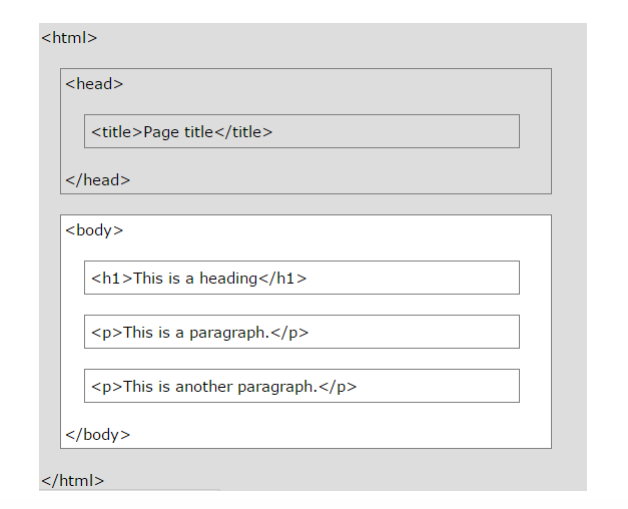
\includegraphics[width=0.6\linewidth]{s2_int_struktura.png}
\end{figure}

Stronę otacza tag \texttt{html} w nim zawarte są dwa podstawowe tagi \texttt{head} i \texttt{body}. \texttt{Head} zawiera metadane dotyczące strony: język, kodowanie, tytuł. Często umieszcza się dam odwołania do plików ze stylami css i skryptami js. W tagu body zawarte są wszystkie tagi związane z zawartością strony.

\subsection{DRZEWO DOM (DOKUMENT OBJECT MODEL)}

\textbf{Cel:}
\begin{itemize}
\item Dostarczenie prostej reprezentacji hierarchii znaczników strony HTML.
\item Dostarczenie modelu umożliwiającego programiście modyfikować, dodawać, usuwać elementy dokumentu .html korzystając z własności drzewa (jego przesukiwania)
\end{itemize}

\textbf{Charakterystyka:}

Dokument HTML możemy przedstawić w postaci drzewa, które rozpoczyna się od tzw. Klasy dokument reprezentującej aktualną stronę Internetową. Zawiera m.in. dane o szerokości i wysokości okna. Do jej atrybutów programista ma dostęp z poziomu języka JavaScript. Obrazek mówi więcej niż tysiąc słów:

\begin{figure}[H]
\centering
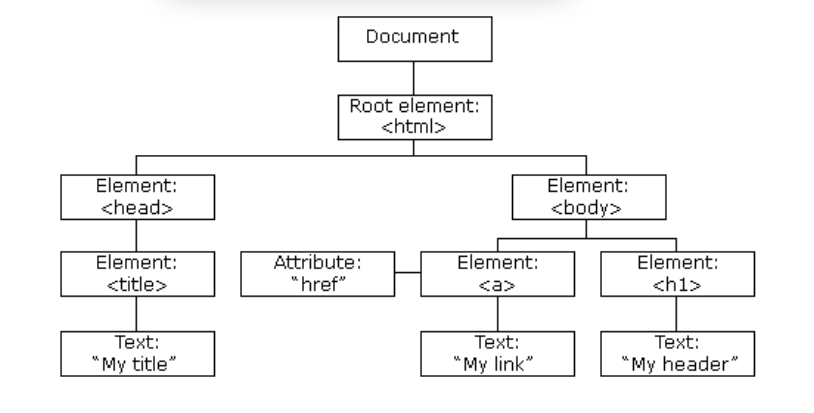
\includegraphics[width=0.9\linewidth]{s2_int_drzewo.png}
\end{figure}

Korzeniem jest tag \texttt{<html>}. Kolejne węzły stanowią tagi zawarte wewnątrz znacznika \texttt{<html>}. Dzieckiem węzła jest tag bezpośrednio zawarty wewnątrz danego tagu. 

\subsection{XHTML extensible Hyper Text Markup Language}

\textbf{Cel:}

Dostarczenie restrykcyjnego standardu rozszerzającego HTML, aby zwiększyć jakość stron internetowych wymagając od programistów poprawnej składni zgodnie z obowiązującym standardem.

\textbf{Charakterystyka:}

Jak już zostało wcześniej wspomniane w języku HTML, gdy programista popełni błąd strona zostanie wyświetlona przez przeglądarkę. Aby, zapewnić poprawność i spójność kodu został stworzony język XHTML. Posiada identyczne tagi i składnię jak w przypadku języka HTML. Jednak tutaj można wymienić kilka istotnych różnic:

\begin{itemize}
\item Jeśli strona XHTML zawiera błędy, nie może zostać wyświetlona;
\item Strony XHTML: \url{http://www.w3.org/1999/xhtml};
\item Element główny (html) musi zawierać atrybut xmlns określający przestrzeń nazw XHTML: \url{http://www.w3.org/1999/xhtml};
\item Znacznikowi otwierającemu każdego niepustego elementu powinien odpowiadać znacznik zamykający (np. \texttt{<li> ... </li>});
\item Puste elementy muszą także być zamykane (np. zamiast \texttt{<br>} musi być \texttt{<br/>}, albo \texttt{<br></br>});
\item Elementy muszą być zagnieżdżane w odpowiedni sposób (np. zamiast \texttt{<p>Tekst z <em>wyróżnieniem</p></em>} -- \texttt{<p>Tekst z <em>wyróżnieniem</em></p>}); wprawdzie w HTML także istniał taki wymóg, lecz nie był egzekwowany przez przeglądarki;
\item Nazwy elementów i atrybutów XHTML muszą być pisane małymi literami;
\item Wszystkie wartości atrybutów muszą być ujęte w cudzysłów (podwójny, np. \texttt{<td rowspan="3">}, albo apostrof, np. \texttt{<td rowspan='3'>});
\item Niedozwolona jest minimalizacja atrybutów (np. zamiast \texttt{<textarea readonly>} musi być \texttt{<textarea readonly="readonly">});
\item XHTML muszą mieć typ zawartości \texttt{application/xhtml+xml} (lub inny XML)
\item Element główny (\texttt{html}) musi zawierać atrybut \texttt{xmlns} określający przestrzeń nazw  
\end{itemize}
